\section{候选覆盖：评分准确仍可能错过好方向}
假设我们知道怎样给替换打分，但只看12个移入方向。如果最有用的方向在第13个之外，再好的打分公式也选不到它。为检验这一点，离线teacher枚举固定154方向字典中的整个初次交换邻域（initial exchange neighborhood）：保留$k$列时，共有$k(154-k)$个一换一组合。无效端点照样记录；完整收益标注在部署完成之后获取，不进入selector。

令每个单元的全字典最大正收益为$Q_*^+=\max(0,\max Q)$。对象内先对这些机会求和，再用anchor选中且通过方向复核的收益之和除以它，得到排序机会捕获率（ranking opportunity capture）。十个完整额外对象为97.30--99.99\%，中位99.54\%。同样计算12候选池内最好收益可覆盖的机会，得到候选覆盖率（candidate opportunity coverage）：49.12--95.31\%，中位72.95\%。零机会不提供权重；未完成对象只有六单元的观察值，不能填成九单元总体。

\begin{figure}[htbp]\centering
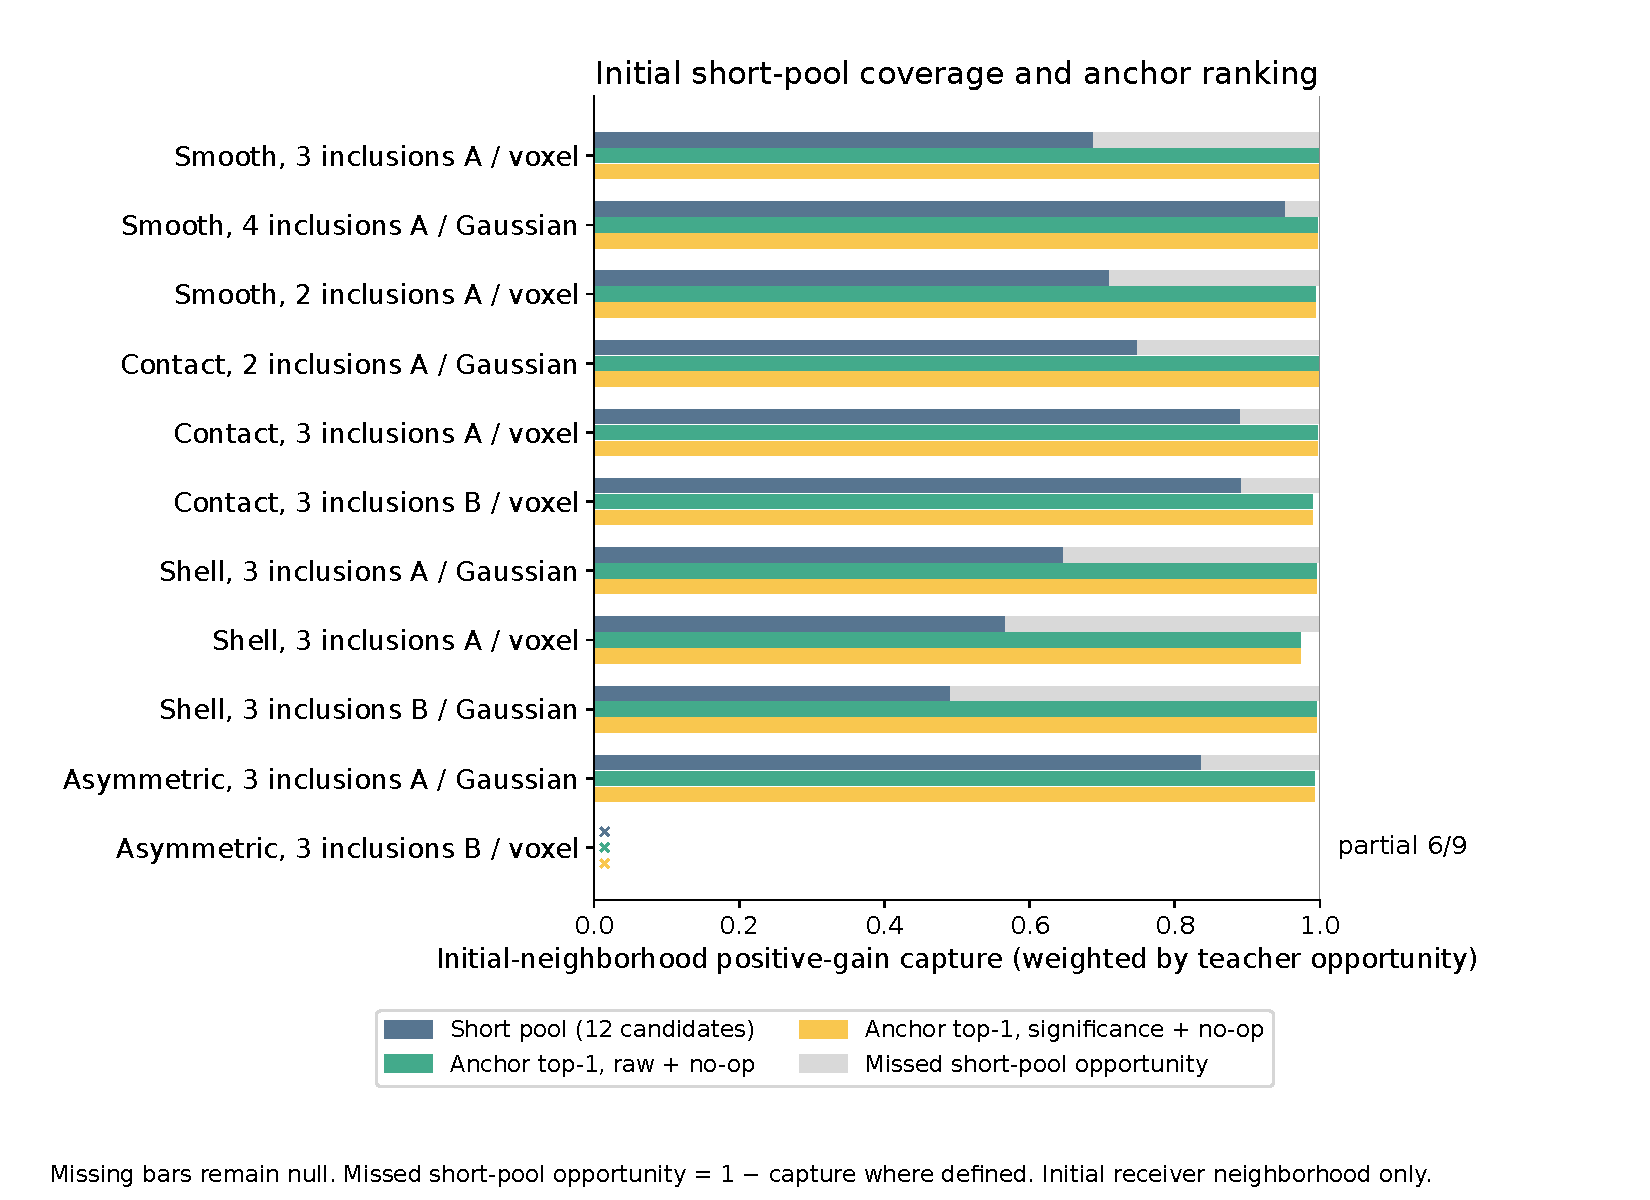
\includegraphics[width=.95\linewidth]{figures/coverage_closure_v2/initial_opportunity.pdf}
\caption{完整字典排序与固定短池覆盖是两个问题。图以对象内正收益求和后的比例呈现，非对称voxel对象的6/9观察结果单独标注。它不是最终重建误差，也不是部署整条路径的收益比例。}
\end{figure}

进一步的离线诊断最多走三个完整收益贪心动作，每次重新枚举当前邻域。它在90个单元得到更低终态gap；线上路径在5个单元更低；1个在评价底噪内相同。即使每一步都看整个字典，局部贪心也不保证全局最好，所以不能把所有终态差距称为“评分误差”。这里应分开三个问题：方向有没有送进来、送来的方向有没有排对、接受以后进入了哪个新邻域。改善候选取得是后续方向，当前冻结规则没有新增网络或再调短池。
